\documentclass[a4paper,12pt]{report}

% --- CẤU HÌNH TIẾNG VIỆT & FONT ---
\usepackage[utf8]{inputenc}
\usepackage[T5]{fontenc} % Bắt buộc cho tiếng Việt
\usepackage[vietnamese]{babel}
\usepackage{lmodern}
\usepackage{mathptmx} % Font giống Times New Roman, gọn gàng hơn cho báo cáo

% --- CÁC GÓI HỖ TRỢ ---
\usepackage{geometry}
\usepackage{amsmath, amssymb, amsfonts}
\usepackage{graphicx}
\graphicspath{{../figures/}}
\usepackage{svg} % Hỗ trợ file SVG
\usepackage{booktabs}
\usepackage{float}
\usepackage{enumitem}
\usepackage{cite}
\usepackage[hyphens]{url} % Hỗ trợ URL trong bibliography với khả năng xuống hàng
\usepackage{xcolor}
\usepackage{titlesec}
\usepackage{caption}
\usepackage[breaklinks=true,colorlinks=true,linkcolor=blue,urlcolor=blue,citecolor=blue]{hyperref} % Cho phép URL xuống hàng

% --- CẤU HÌNH URL ---
\def\UrlBreaks{\do\/\do\-\do\.\do\=\do\?\do\&} % Cho phép URL break tại các ký tự này
\urlstyle{same} % Giữ nguyên font như văn bản

% --- CẤU HÌNH TRANG ---
\geometry{left=2.5cm, right=2.5cm, top=2.5cm, bottom=2.5cm}
\linespread{1.2} % Giãn dòng 1.2 cho thoáng, dễ đọc
\setlength{\parskip}{6pt} % Khoảng cách giữa các đoạn văn

% Dùng section làm cấp cao nhất trong lớp report (tránh đánh số 0.x)
\renewcommand{\thesection}{\arabic{section}}

% Nạp các chỉ số thống kê được sinh tự động từ pipeline EDA
% dummy stats file
\newcommand{\digitTotal}{60000}
\newcommand{\digitCountZero}{5923}


\begin{document}

% --- TRANG BÌA ---
\begin{titlepage}
    \centering
    
    % Logo trường (Nếu bạn có file logo.png thì bỏ comment dòng dưới)
    % 
\includegraphics[width=0.25\textwidth]{logo.png} 
    \vspace{0.5cm}
    
    % Tên trường
    {\large \textbf{ĐẠI HỌC QUỐC GIA THÀNH PHỐ HỒ CHÍ MINH}}\\
    {\large \textbf{TRƯỜNG ĐẠI HỌC KHOA HỌC TỰ NHIÊN}}\\
    
    \vspace{0.3cm}
    \rule{0.6\textwidth}{0.5pt}
    \vspace{1cm}
    
    % Môn học
    {\Large \textbf{BÁO CÁO MÔN HỌC}}\\
    \vspace{0.3cm}
    {\LARGE \textbf{THỊ GIÁC MÁY TÍNH}}
    
    \vspace{2cm}

    
\begin{figure}[H]
    \centering
    % Đảm bảo bạn có file architecture.png trong thư mục dự án
    
\includegraphics[width=0.3\linewidth]{logo.png} 
\end{figure}
    
    
    % Đề tài
    \begin{minipage}{0.9\textwidth}
        \centering
        {\LARGE \textbf{CÀI ĐẶT VÀ PHÂN TÍCH THUẬT TOÁN ANN TRÊN CÁC TẬP DỮ LIỆU MNIST}}
    \end{minipage}

    \vfill

    \vspace{1cm}
    
    \begin{minipage}{\textwidth}
        \centering
        {\large \textbf{Giảng viên hướng dẫn:}}
        \vspace{0.3cm}
        {\large {TS. Võ Hoài Việt}}
    \end{minipage}
    
    % Thông tin sinh viên và giảng viên
    \begin{minipage}{\textwidth}
        \centering
        {\large \textbf{Sinh viên thực hiện:}}\\
        \vspace{0.3cm}
        {Lê Anh Duy (23127011)}
    \end{minipage}
    
    \vspace{1.5cm}
    
    % Thời gian
    {\large Thành phố Hồ Chí Minh, \today}
    
\end{titlepage}

% --- MỤC LỤC ---
\newpage
\listoffigures
\newpage
\listoftables
\newpage
\tableofcontents
\newpage

\section{Giới thiệu}
\subsection{Mục tiêu}
Bài toán đặt ra là phân loại ảnh xám 28$\times$28 thuộc ba miền dữ liệu (Digit MNIST, Fashion MNIST, PneumoniaMNIST) bằng mô hình ANN cơ bản, sau đó đề xuất các cải tiến và so sánh hiệu quả.

Các Notebook thực nghiệm:
\begin{itemize}
    \item \href{https://github.com/Le-Anh-Duy/CV-HOMEWORK-2-Mnist-EDA/blob/main/notebooks/HW2_Digit_Enhance_clean.ipynb}{HW2\_Digit\_Enhance\_clean.ipynb}
    \item \href{https://github.com/Le-Anh-Duy/CV-HOMEWORK-2-Mnist-EDA/blob/main/notebooks/HW2_Fashion_Enhance_clean.ipynb}{HW2\_Fashion\_Enhance\_clean.ipynb}
    \item \href{https://github.com/Le-Anh-Duy/CV-HOMEWORK-2-Mnist-EDA/blob/main/notebooks/HW2_Med_Enhance_clean.ipynb}{HW2\_Med\_Enhance\_clean.ipynb}
    \item \href{https://github.com/Le-Anh-Duy/CV-HOMEWORK-2-Mnist-EDA/tree/main/notebooks}{Thư mục notebooks (tổng hợp)}
\end{itemize}

\subsection{Ba bộ dữ liệu}
\begin{itemize}
    \item \textbf{Digit MNIST:} 10 lớp chữ số viết tay.
    \item \textbf{Fashion MNIST:} 10 lớp trang phục.
    \item \textbf{PneumoniaMNIST:} 2 lớp (Normal/Pneumonia) ảnh X-quang ngực.
\end{itemize}

\subsection{ANN là gì và vì sao chọn ANN}
ANN (Artificial Neural Network) là mô hình truyền thẳng nhiều lớp ánh xạ vector đầu vào thành nhãn lớp. ANN đơn giản, dễ huấn luyện, cho phép tạo baseline rõ ràng để so sánh các cải tiến về đặc trưng, dữ liệu và tối ưu hóa.

\section{Dữ liệu và tiền xử lý}
\subsection{Mô tả dữ liệu}
Bảng \ref{tab:raw-dataset-summary} tóm tắt kích thước và số lượng mẫu gốc của ba tập dữ liệu.


\begin{table}[H]
    \centering
    \caption{Tổng quan thông số gốc của các tập dữ liệu (trước chuẩn hóa)}
    \label{tab:raw-dataset-summary}
    \begin{tabular}{lrrrrl}
        \toprule
        \textbf{Dataset} & \textbf{Train} & \textbf{Test} & \textbf{Classes} & \textbf{Size} & \textbf{Value range} \\
        \midrule
        Digit MNIST & 60000 & 10000 & 10 & 28$\times$28 & [0,255] \\
        Fashion MNIST & 60000 & 10000 & 10 & 28$\times$28 & [0,255] \\
        PneumoniaMNIST & 4708 & 624 & 2 & 28$\times$28 & [0,255] \\
        \bottomrule
    \end{tabular}
\end{table}

\subsection{Tiền xử lý}
\begin{itemize}
    \item Chuẩn hóa điểm ảnh về $[0,1]$ bằng cách chia 255.
    \item Làm phẳng ảnh 28$\times$28 thành vector 784 chiều để đưa vào ANN.
    \item Dùng split train/test gốc của từng tập;
\end{itemize}

\subsection{Insight từ EDA}
\begin{itemize}
    \item Digit và Fashion MNIST có phân phối các lớp tương đối cân bằng.
    \item PneumoniaMNIST mất cân bằng mạnh giữa hai lớp.
    \item Tín hiệu Pneumonia thiên về \textit{texture} hơn \textit{shape}; độ biến thiên nội bộ cao.
\end{itemize}

\subsection{Minh họa dữ liệu}
\begin{figure}[H]
    \centering
    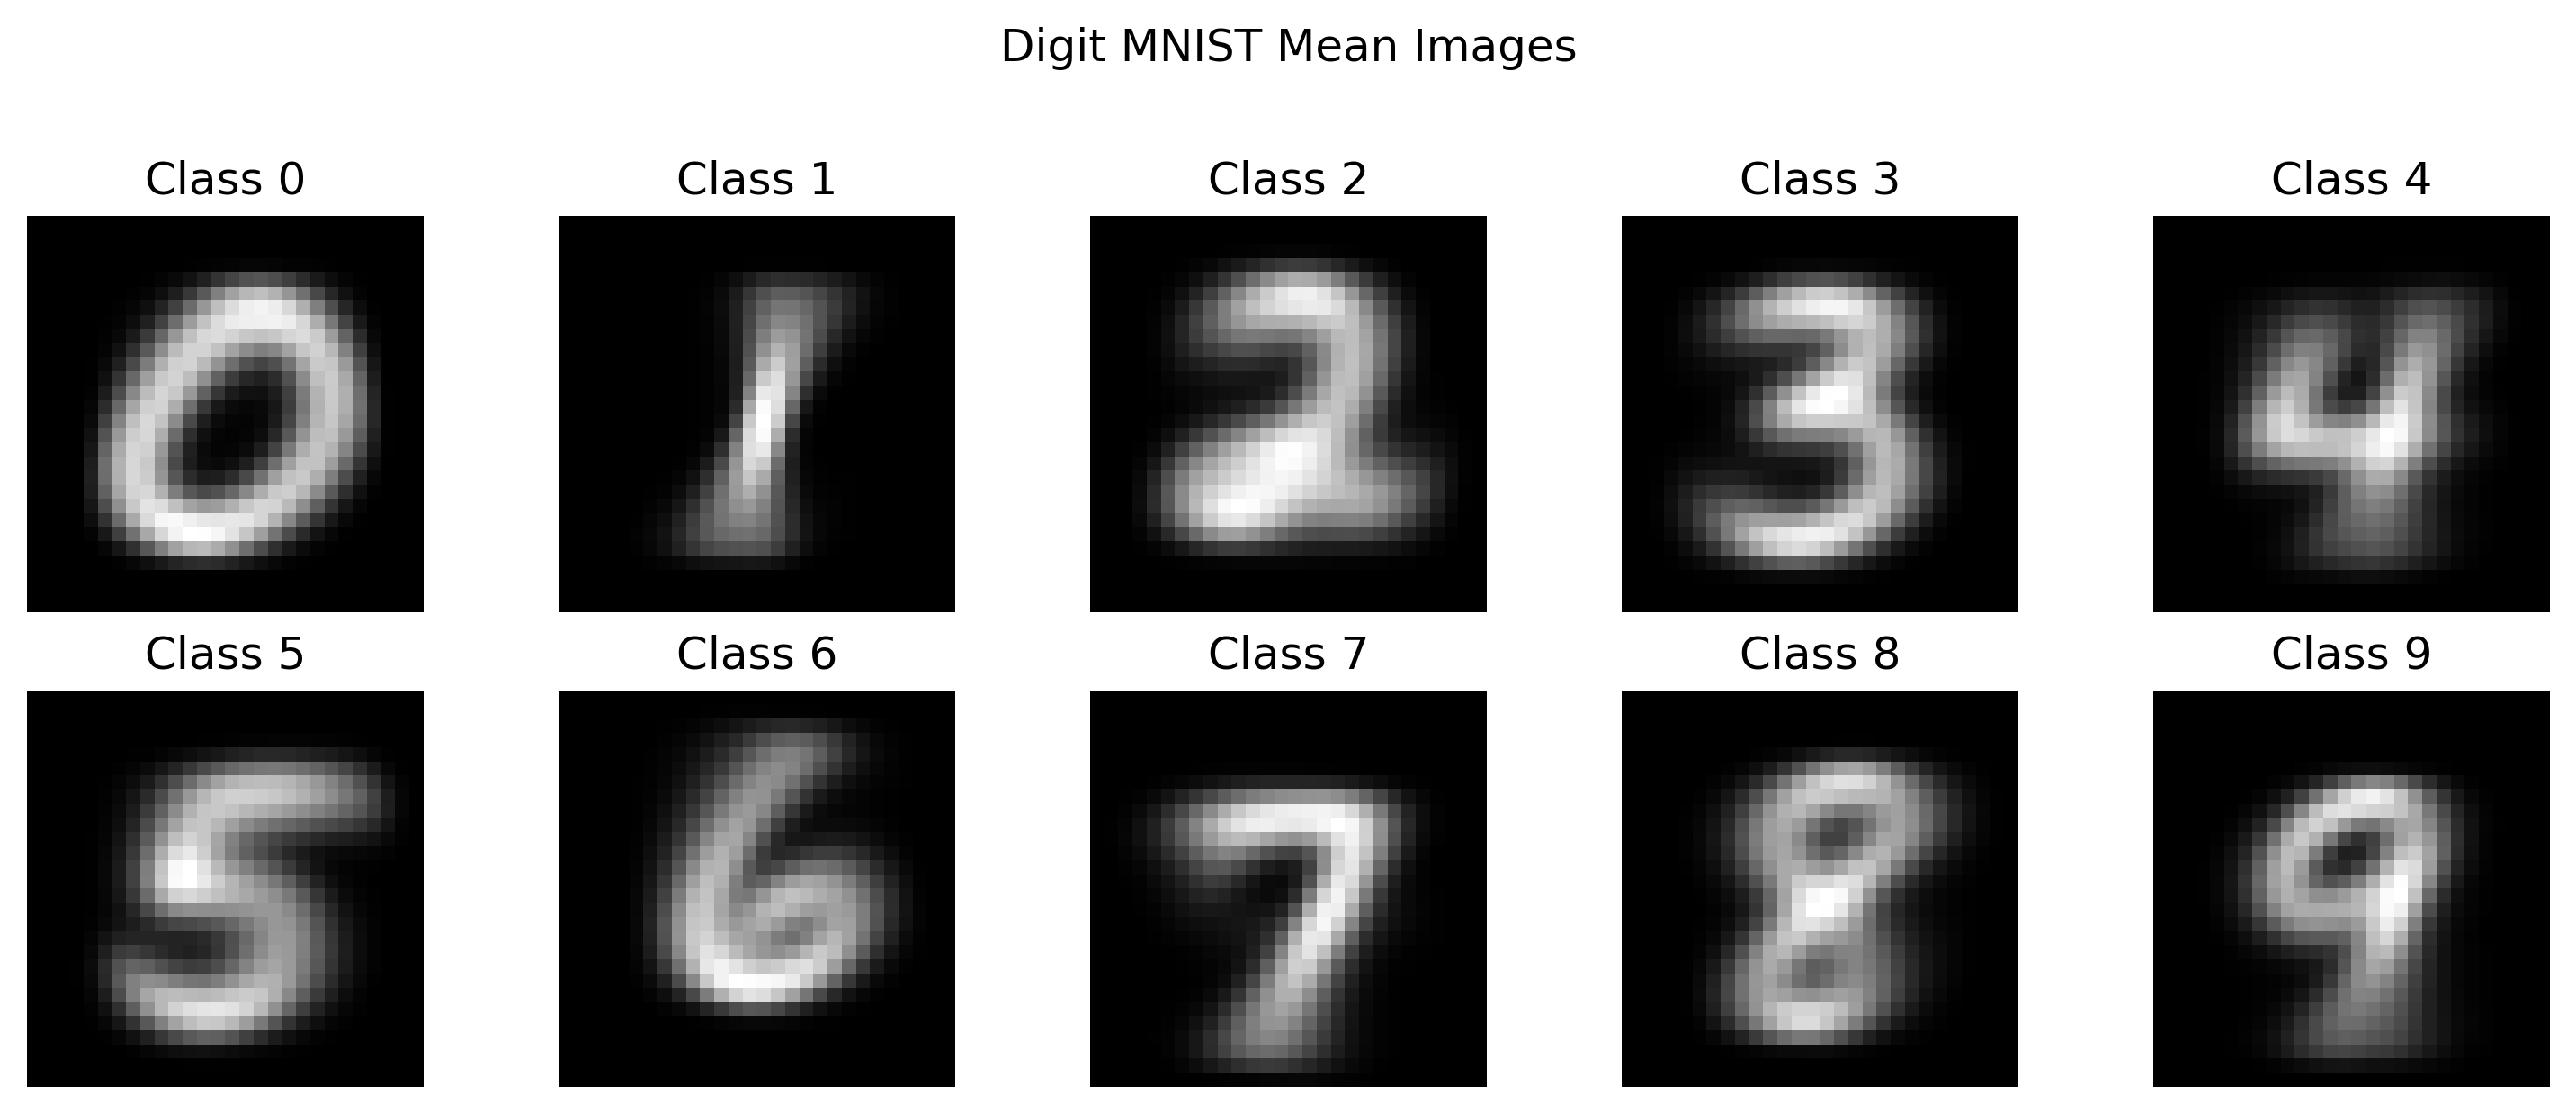
\includegraphics[width=0.28\linewidth]{mean_digit.png}
    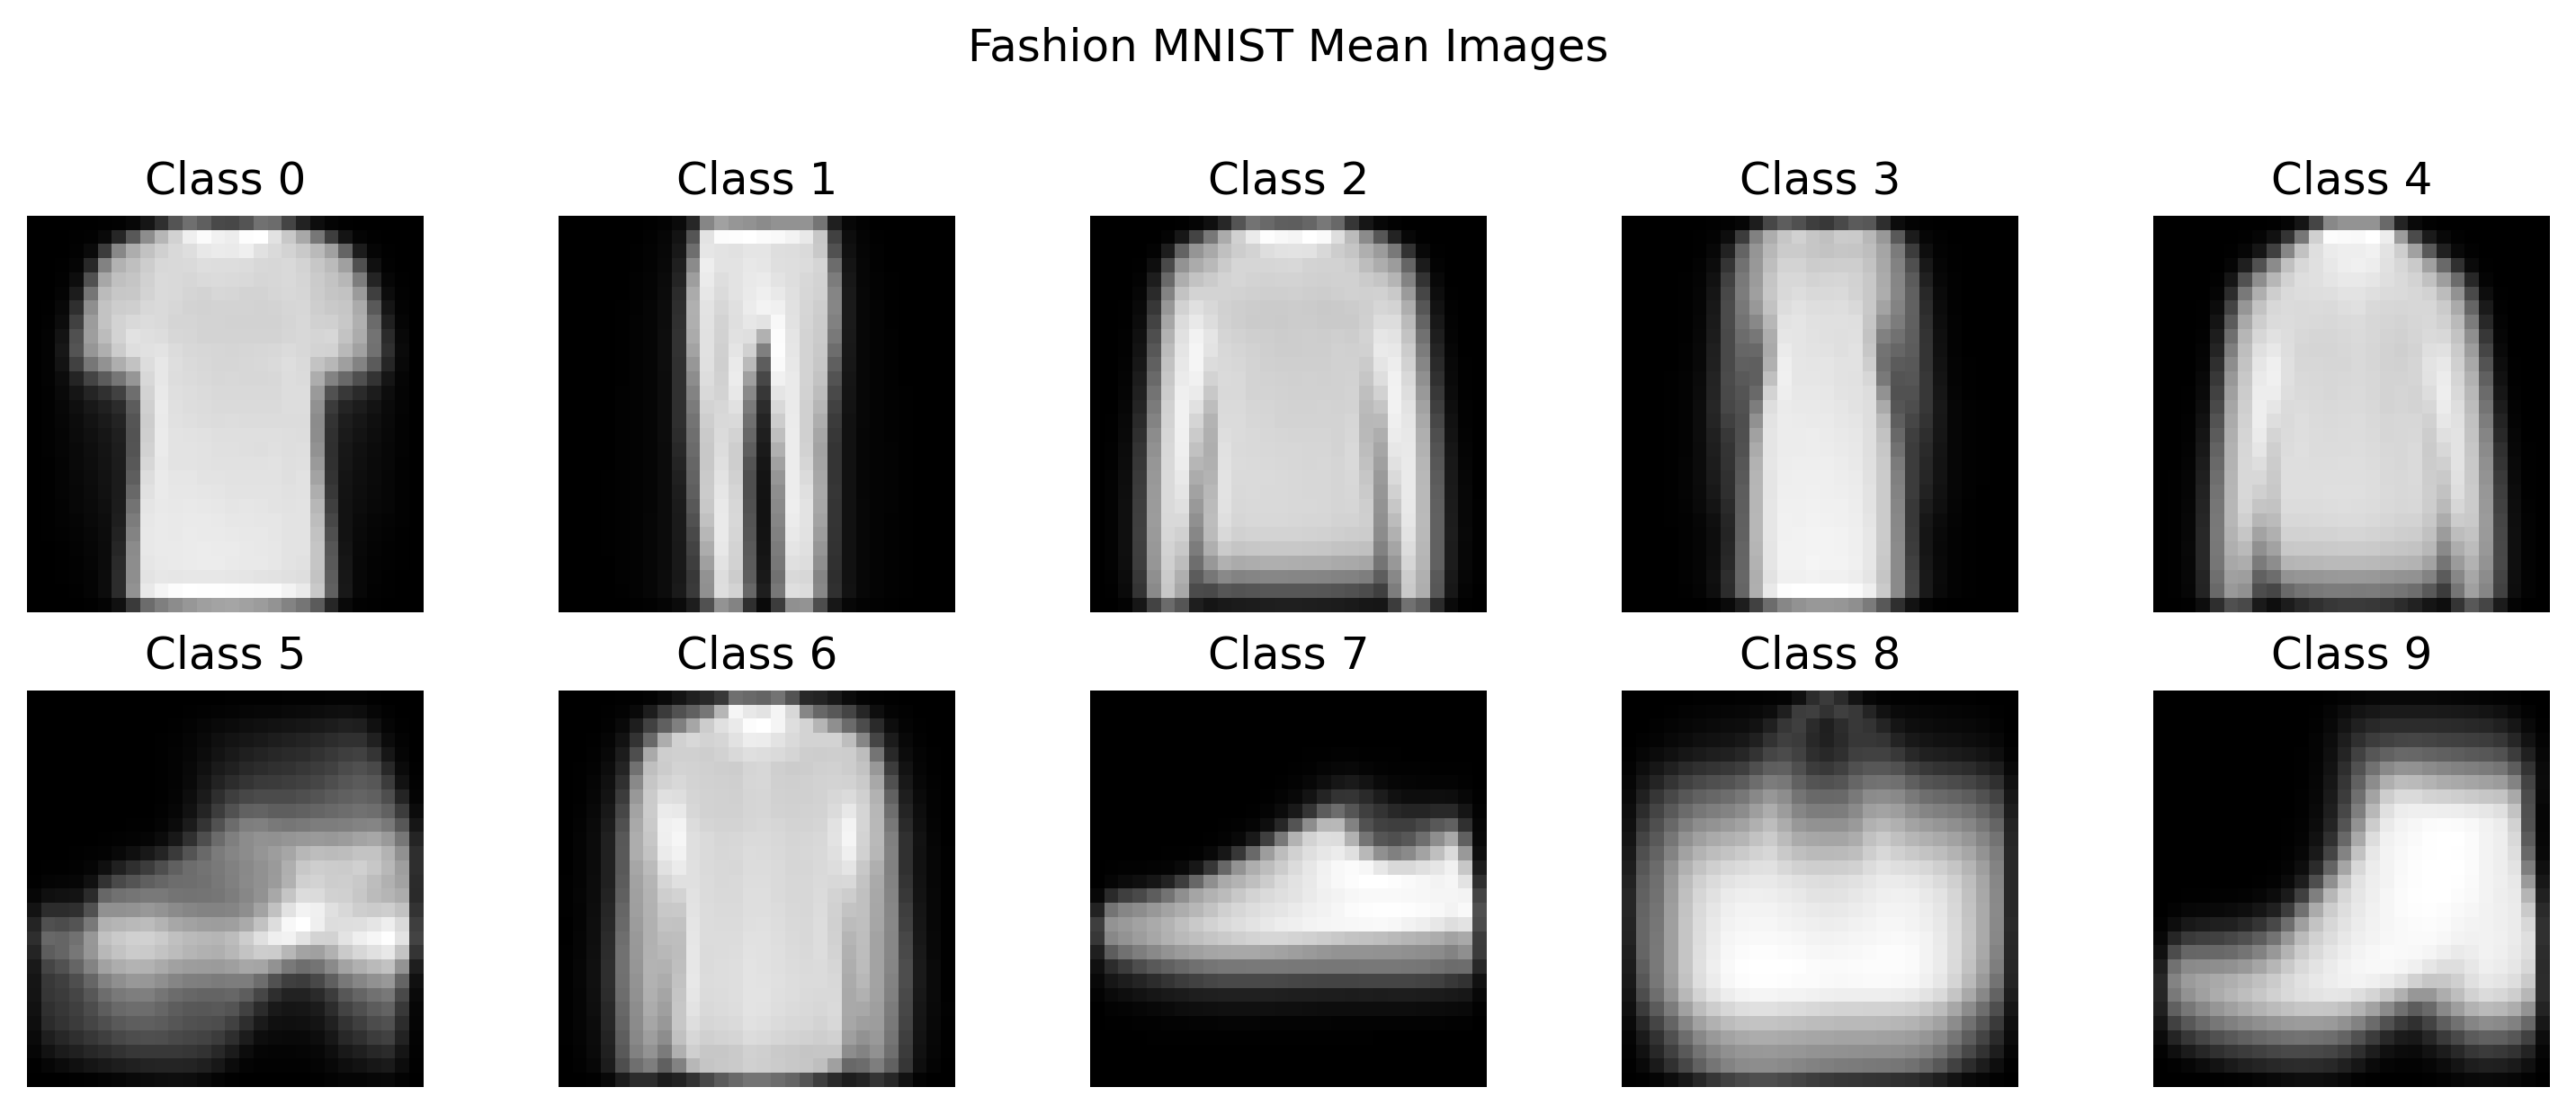
\includegraphics[width=0.28\linewidth]{mean_fashion.png}
    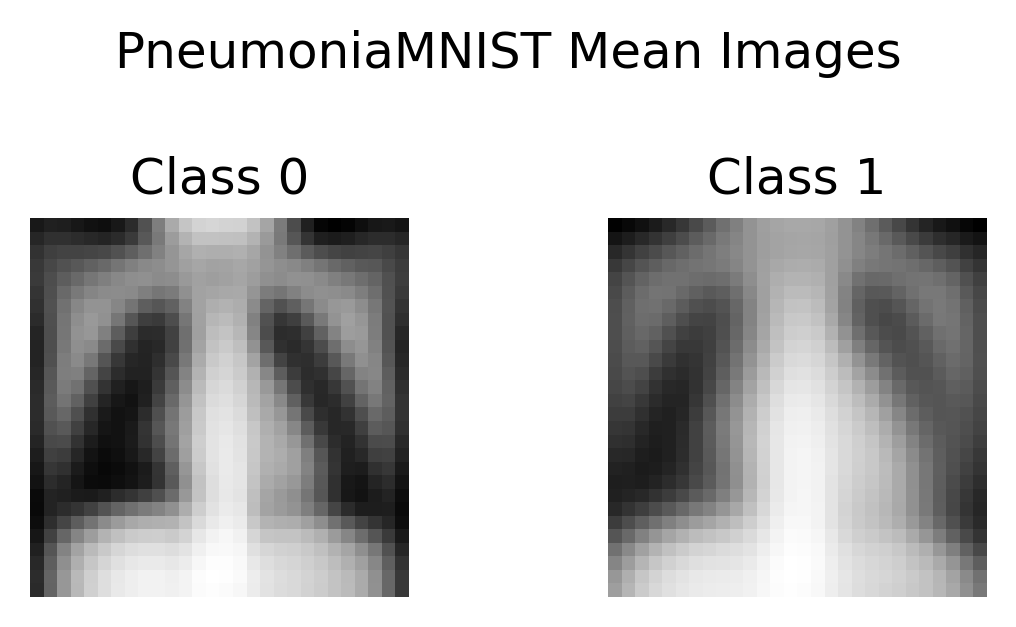
\includegraphics[width=0.28\linewidth]{mean_pneumonia.png}
    \caption{Ảnh trung bình của từng miền dữ liệu (Digit/Fashion/Pneumonia)}
    \label{fig:mean-samples}
\end{figure}

\begin{figure}[H]
    \centering
    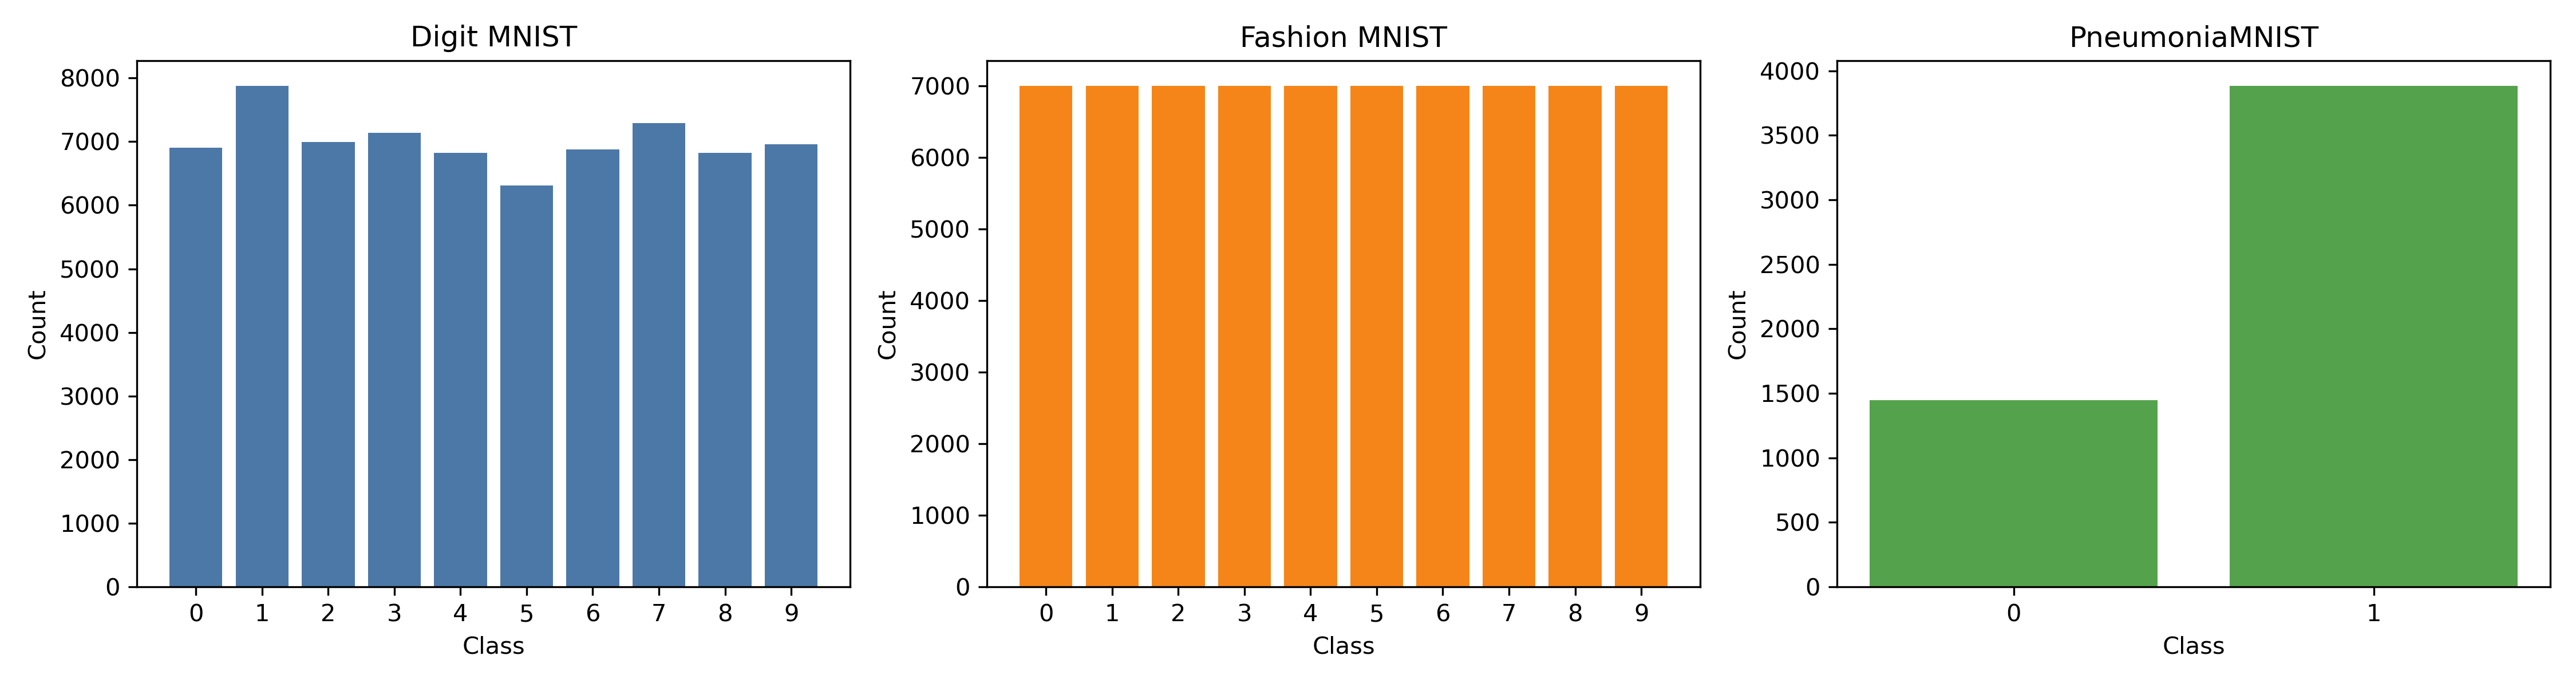
\includegraphics[width=0.65\linewidth]{label_distribution.png}
    \caption{Phân bố nhãn của ba tập dữ liệu}
    \label{fig:label-distribution}
\end{figure}

\section{Mô hình baseline}
\subsection{Kiến trúc (Vanilla Baseline)}
\textbf{Vanilla Baseline} là ANN thuần chỉ gồm các khối \texttt{Linear $\rightarrow$ ReLU} lặp lại (không BatchNorm, không Dropout), đầu vào là raw pixels. Cấu hình sử dụng trong báo cáo: 784 $\rightarrow$ 256 $\rightarrow$ 128 $\rightarrow$ $C$ (với $C=10$ cho Digit/Fashion và $C=2$ cho Pneumonia).

\subsection{Cải tiến kiến trúc cơ sở (Strong Baseline)}
\textbf{Strong Baseline} là Vanilla Baseline được bổ sung BatchNorm và/hoặc Dropout để ổn định huấn luyện (không thay đổi input raw pixels). Cụ thể: FashionMNIST dùng BatchNorm sau mỗi Linear ở các tầng ẩn (trước ReLU); PneumoniaMNIST dùng BatchNorm sau mỗi Linear và Dropout ngay sau ReLU ở các tầng ẩn. Các kết quả Strong Baseline được trình bày trong từng mục dữ liệu để tạo luồng so sánh: \textit{Vanilla Baseline $\rightarrow$ Strong Baseline $\rightarrow$ Strong Baseline + Feature Engineering}.

\subsection{Activation}
Sử dụng ReLU ở các tầng ẩn, tầng cuối là tuyến tính (logits).

\subsection{Loss và Optimizer}
\begin{itemize}
    \item Loss: \texttt{CrossEntropyLoss}.
    \item Optimizer: Adam.
\end{itemize}

\subsection{Hyperparameters và quy trình huấn luyện}

\textbf{Huấn luyện Vanilla Baseline:} Epochs từ 100-600, learning rate = 0.001, huấn luyện theo full-batch (flatten toàn bộ tập huấn
luyện trước khi tối ưu).

\noindent \textbf{Huấn luyện các mô hình cải tiến:} learning rate = 0.001, batch size = \{2048, 4096, ...\}, dùng quy trình CustomDataset + DataLoader và transform tương ứng; số epoch thường trong khoảng 30--50. Trong đó có các mô hình được huấn luyện với nhiều mức learning rate khác nhau, các quá trình huấn luyện được điều chỉnh tham số thủ công để đạt được kết quả tốt nhất.

\section{Kết quả baseline}
\subsection{Bảng kết quả}
\begin{table}[H]
    \centering
    \caption{Kết quả baseline (test set)}
    \label{tab:baseline-metrics}
    \begin{tabular}{lrrrr}
        \toprule
        \textbf{Dataset} & \textbf{Accuracy} & \textbf{F1} & \textbf{Precision} & \textbf{Recall} \\
        \midrule
        Digit MNIST & \textbf{0.9438} & \textbf{0.9437} & \textbf{0.9437} & 0.9438 \\
        Fashion MNIST & 0.8443 & 0.8425 & 0.8429 & 0.8443 \\
        PneumoniaMNIST & 0.8349 & 0.8817 & 0.7983 & \textbf{0.9846} \\
        \bottomrule
    \end{tabular}
\end{table}

\textit{Lưu ý:} Bảng này là \textbf{Vanilla Baseline} (ANN thuần, không BatchNorm/Dropout) lấy từ notebook baseline\_training\_inferencing. Strong Baseline (có BatchNorm/Dropout) được trình bày riêng trong từng bộ dữ liệu.

\subsection{Nhận xét}
Digit MNIST đạt kết quả tốt nhất; Fashion khó hơn do hình dạng đa dạng và chồng lấn giữa các lớp. PneumoniaMNIST có phân bố các lớp bị lệch nên cần theo dõi đồng thời Precision/Recall thay vì chỉ Accuracy.

Từ baseline có thể thấy ba bộ dữ liệu đặt ra ba khó khăn khác nhau: Digit chủ yếu là bài toán hình dạng đơn giản; Fashion khó hơn do chồng lấn hình dáng giữa các lớp; Pneumonia khó vì tín hiệu không rõ ràng và có mất cân bằng lớp. Vì vậy, các cải tiến ở phần sau được thiết kế riêng theo từng loại lỗi thay vì áp dụng đồng nhất.

\section{Các cải tiến theo từng bộ dữ liệu}
\subsection{Digit MNIST}
\subsubsection{Phân tích kết quả}
Vanilla Baseline đạt Accuracy 0.9438, cho thấy raw pixels đã đủ mạnh cho phần lớn trường hợp. Tuy nhiên, các mẫu sai còn lại chủ yếu là chữ số nét mờ, biến dạng hoặc hình dáng gần nhau, cho thấy raw pixels chưa biểu diễn tốt cấu trúc nét viết ở các trường hợp khó (Ví dụ 8 và 3, 4 và 9) 


\subsubsection{Động lực cải tiến}
Vì bài toán phân biệt chữ số phụ thuộc mạnh vào hình dạng và hướng viết (có thể biểu diễn tốt bằng hướng gradient), tôi đặt giả thuyết rằng các đặc trưng mô tả được cấu trúc của cạnh sẽ phù hợp hơn raw pixels. Do đó HOG được chọn làm cải tiến đầu tiên. Ngoài ra, vì chữ số viết tay có nhiều biến biến thể tự nhiên về độ nghiêng, vị trí và tỉ lệ, nên dù cho tập MNIST ban đầu có thẳng thế nào, thì việc thực hiện tăng cường dữ liệu nhẹ được kỳ vọng sẽ giúp mô hình tổng quát hóa tốt hơn trên các mẫu khó.

\subsubsection{Cải tiến và kết quả}
\textbf{Thông số augmentation (Digit):} RandomRotation $\pm 10^{\circ}$, RandomAffine với translate $(0.1, 0.1)$ (xấp xỉ $\pm 2$--$3$ px trên ảnh $28\times28$), và scale $(0.9, 1.1)$.
\begin{itemize}
    \item HOG (cell 4$\times$4, block 8$\times$8, stride 4$\times$4, 9 bins; tạo ra vector 1296 chiều) + ANN với kiến trúc 1296 $\rightarrow$ 512 $\rightarrow$ 256 $\rightarrow$ 128 $\rightarrow$ 10 (input 1296, output 10 lớp) nâng Accuracy lên 0.9808.\footnote{OpenCV HOGDescriptor: \url{https://docs.opencv.org/4.x/d5/d33/structcv_1_1HOGDescriptor.html}}
    \item Augmentation + BatchNorm trên HOG dùng ANN cùng kích thước input/output (1296 $\rightarrow$ 512 $\rightarrow$ 256 $\rightarrow$ 128 $\rightarrow$ 10); BatchNorm đặt sau các lớp Linear ở từng tầng ẩn (fc1, fc2, fc3), trước ReLU. Đạt Accuracy 0.9939.
\end{itemize}

\subsubsection{Thảo luận}
HOG xác nhận giả thuyết rằng đặc trưng gradient phù hợp cho shape đơn giản; tăng cường dữ liệu nhẹ cũng cải thiện độ bền vững trước biến thiên hình học. Digit là bộ dữ liệu mà ANN phù hợp nhất trong ba bộ dữ liệu. Learning curve cho thấy loss giảm nhanh và accuracy bão hòa sớm, phản ánh quá trình hội tụ ổn định. Ở best model, dao động theo epoch nhỏ, cho thấy huấn luyện ít nhiễu.

\begin{figure}[H]
    \centering
    \begin{minipage}{0.48\linewidth}
        \centering
        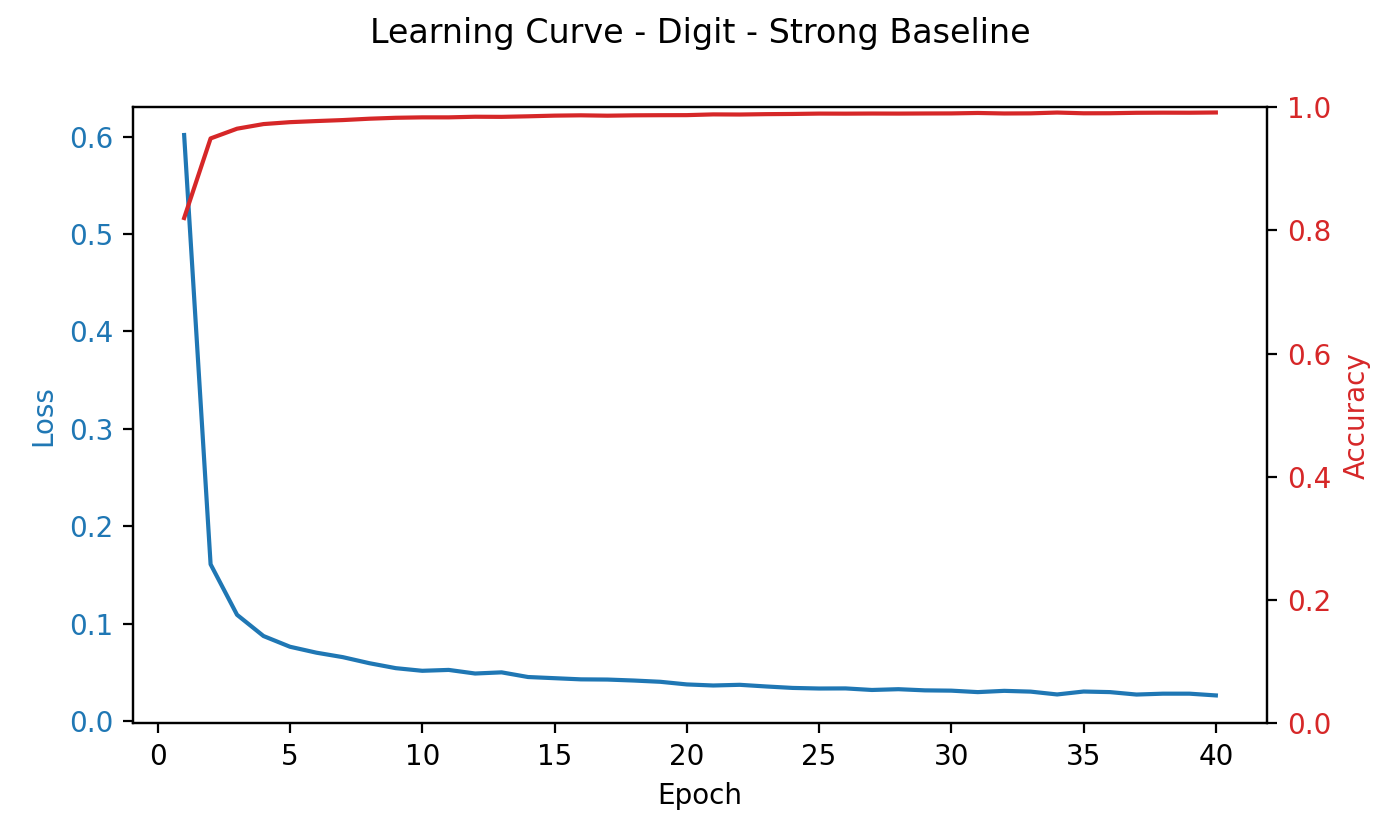
\includegraphics[width=\linewidth]{learning_curve_digit_strong.png}
        \caption*{Strong baseline}
    \end{minipage}
    \hfill
    \begin{minipage}{0.48\linewidth}
        \centering
        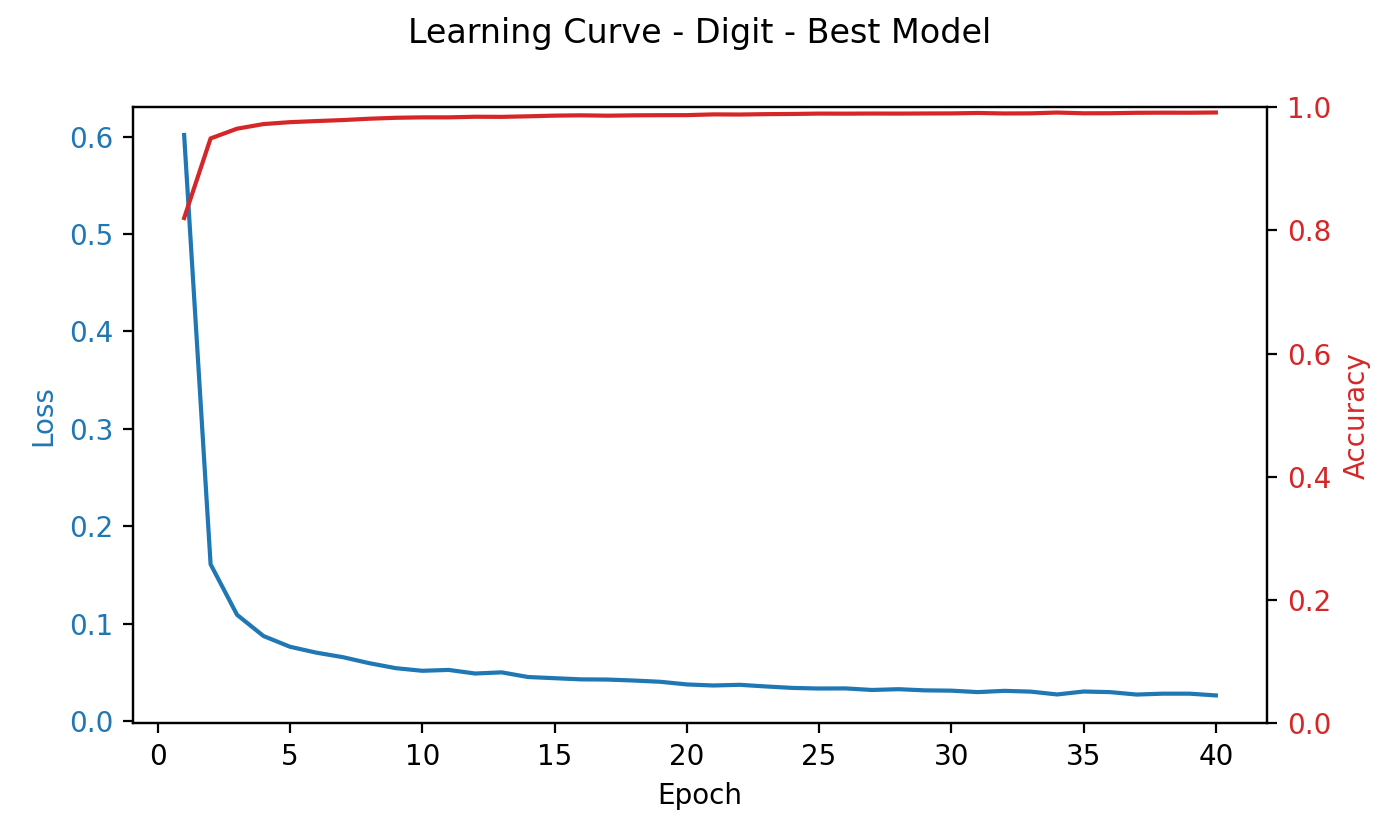
\includegraphics[width=\linewidth]{learning_curve_digit_best.png}
        \caption*{Best model}
    \end{minipage}
    \caption{Learning curve (Loss/Accuracy) cho Digit MNIST: strong baseline vs. best model}
    \label{fig:digit-learning-curve}
\end{figure}

\textbf{Minh họa lỗi}
Mặc dù Accuracy đạt xấp xỉ 99\%, vẫn còn một số ảnh bị phân loại sai. Notebook clean đã trực quan hóa các mẫu sai (true vs. predicted) để minh họa các trường hợp khó, thường là chữ số viết tay bị nhiễu hoặc nét mờ, thậm chí còn có những mẫu mắt thường không phân biệt được. (xem Hình~\ref{fig:digit-misclassified} và Hình~\ref{fig:digit-cm-best}).

\begin{figure}[H]
    \centering
    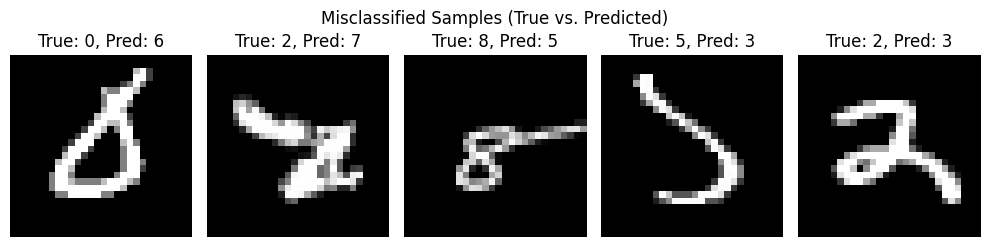
\includegraphics[width=0.7\linewidth]{ann_digit_missclassify.png}
    \caption{Các mẫu Digit MNIST bị phân loại sai (true vs. predicted)}
    \label{fig:digit-misclassified}
\end{figure}

\begin{figure}[H]
    \centering
    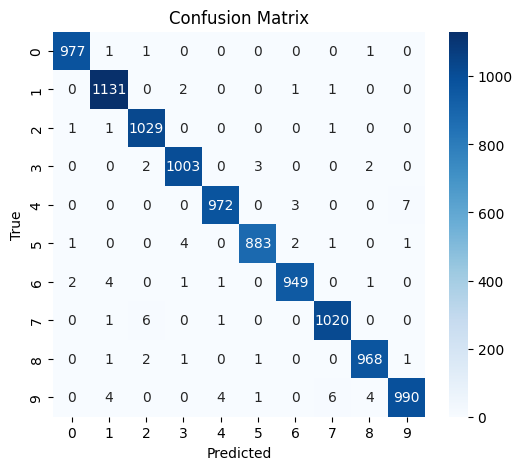
\includegraphics[width=0.55\linewidth]{ann_confusion_matrix_best_digit.png}
    \caption{Ma trận nhầm lẫn của mô hình tốt nhất cho Digit MNIST}
    \label{fig:digit-cm-best}
\end{figure}

\subsection{Fashion MNIST}
\subsubsection{Phân tích kết quả}
Vanilla Baseline đạt 0.8443, thấp hơn đáng kể so với Digit. Strong Baseline đạt 0.8814. Minh họa các mẫu bị nhận diện sai cho thấy lỗi tập trung ở các cặp lớp có hình dáng gần nhau, như 7 và 9 (Sneaker vs Ankle boot) hay 6 và 0 (Shirt vs T-shirt/top). Giả thuyết đặt ra là pixel raw ban đầu chưa đủ để mô tả sự khác biệt giữa các lớp có hình dáng gần giống nhau, nên sẽ cần những feature có thể phân biệt hình dáng tốt hơn.

\begin{figure}[H]
    \centering
    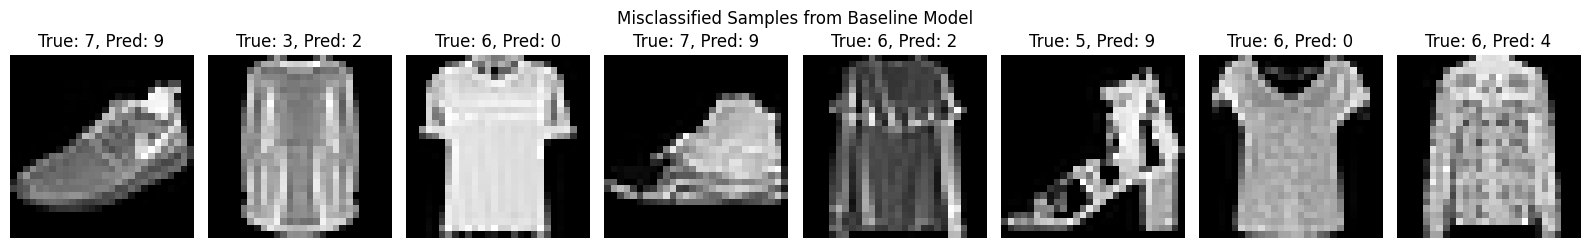
\includegraphics[width=0.95\linewidth]{ann_fashion_miss_classify.png}
    \caption{Các mẫu Fashion MNIST bị phân loại sai từ baseline (true vs. predicted)}
    \label{fig:fashion-misclassified}
\end{figure}

\subsubsection{Động lực cải tiến}
Từ quan sát trên tôi đưa ra hai giả thuyết. Thứ nhất, tăng cường thông tin biên và hướng gradient sẽ giúp ANN phân biệt các loại trang phục tốt hơn; do đó Sobel, Canny và HOG được thử. Thứ hai, augmentation có thể giúp mô hình tổng quát tốt hơn, nhưng cần kiểm soát vì ảnh FashionMNIST vốn được căn giữa và ít biến thiên hình học (như đã qua sát ở các mẫu).

\subsubsection{Cải tiến và kết quả}
\begin{itemize}
    \item HOG + ANN 1296 $\rightarrow$ 512 $\rightarrow$ 256 $\rightarrow$ 128 $\rightarrow$ 10 (input 1296, output 10 lớp) cho Accuracy 0.9217 (F1 0.9213, Precision 0.9211, Recall 0.9217).\footnote{OpenCV HOGDescriptor: \url{https://docs.opencv.org/4.x/d5/d33/structcv_1_1HOGDescriptor.html}}
    \item Sobel + ANN 784 $\rightarrow$ 512 $\rightarrow$ 256 $\rightarrow$ 128 $\rightarrow$ 10 (input 784, output 10 lớp) đạt Accuracy 0.8934 (F1 0.8931, Precision 0.8951, Recall 0.8934).
    \item Canny/auto-edge + ANN 784 $\rightarrow$ 512 $\rightarrow$ 256 $\rightarrow$ 128 $\rightarrow$ 10 đạt Accuracy 0.8495 (F1 0.8487, Precision 0.8484, Recall 0.8495).
    % \item Chiến lược huấn luyện theo hai giai đoạn trên raw pixels, ANN 784 $\rightarrow$ 512 $\rightarrow$ 256 $\rightarrow$ 128 $\rightarrow$ 10 (input 784, output 10 lớp): Accuracy 0.9031.
\end{itemize}

\begin{figure}[H]
    \centering
    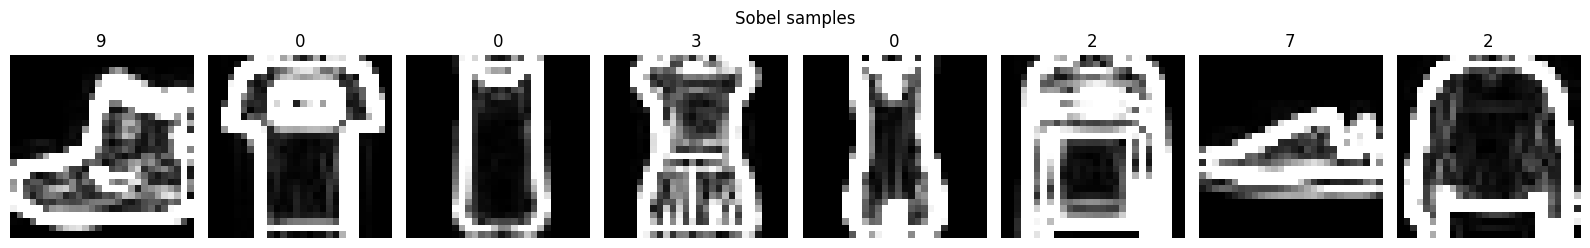
\includegraphics[width=0.8\linewidth]{ann_fashion_sobel_samples.png}
    \caption{Ví dụ ảnh Fashion MNIST sau Sobel}
    \label{fig:fashion-sobel-samples}
\end{figure}

\begin{figure}[H]
    \centering
    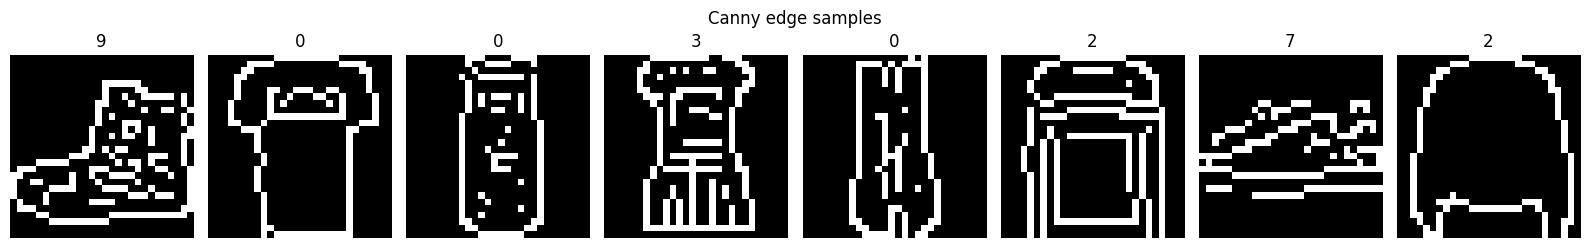
\includegraphics[width=0.9\linewidth]{ann_fashion_canny_samples.png}
    \caption{Ví dụ ảnh Fashion MNIST sau Canny (biên gắt, mất thông tin nội dung)}
    \label{fig:fashion-canny-samples}
\end{figure}

\subsubsection{Thảo luận}
Kết quả xác nhận rằng FashionMNIST thiên về hình dáng và cấu trúc; HOG phù hợp hơn raw pixels và edge map nhị phân. Canny/auto-edge cho kết quả khá tốt nhưng dễ overfitting vì nhị phân hóa biên làm giảm thông tin cường độ, khiến mô hình nhạy với nhiễu và thay đổi nhỏ. Tăng cường dữ liệu chỉ hữu ích khi phản ánh đúng biến thiên tự nhiên của dữ liệu, điều mà ở tập fashion không cần vì dữ liệu không có điều kiện nghiêng như digit, nên hiệu quả không mạnh như ở Digit. Learning curve cho thấy quá trình hội tụ chậm hơn Digit, accuracy tăng đều rồi bão hòa muộn hơn. Best model (HOG) đạt plateau cao hơn strong baseline, nhất quán với kết quả định lượng.

\begin{figure}[H]
    \centering
    \begin{minipage}{0.48\linewidth}
        \centering
        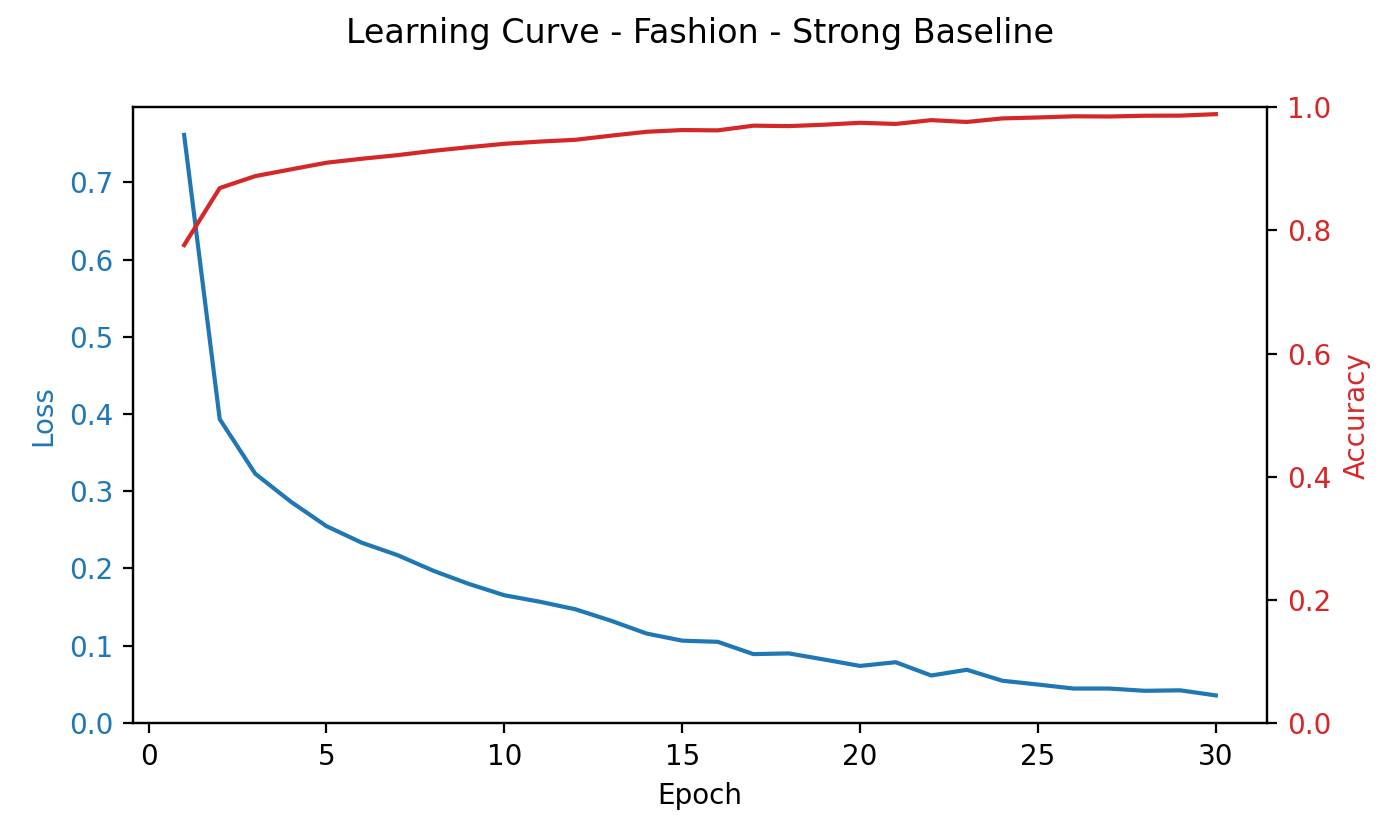
\includegraphics[width=\linewidth]{learning_curve_fashion_strong.png}
        \caption*{Strong baseline}
    \end{minipage}
    \hfill
    \begin{minipage}{0.48\linewidth}
        \centering
        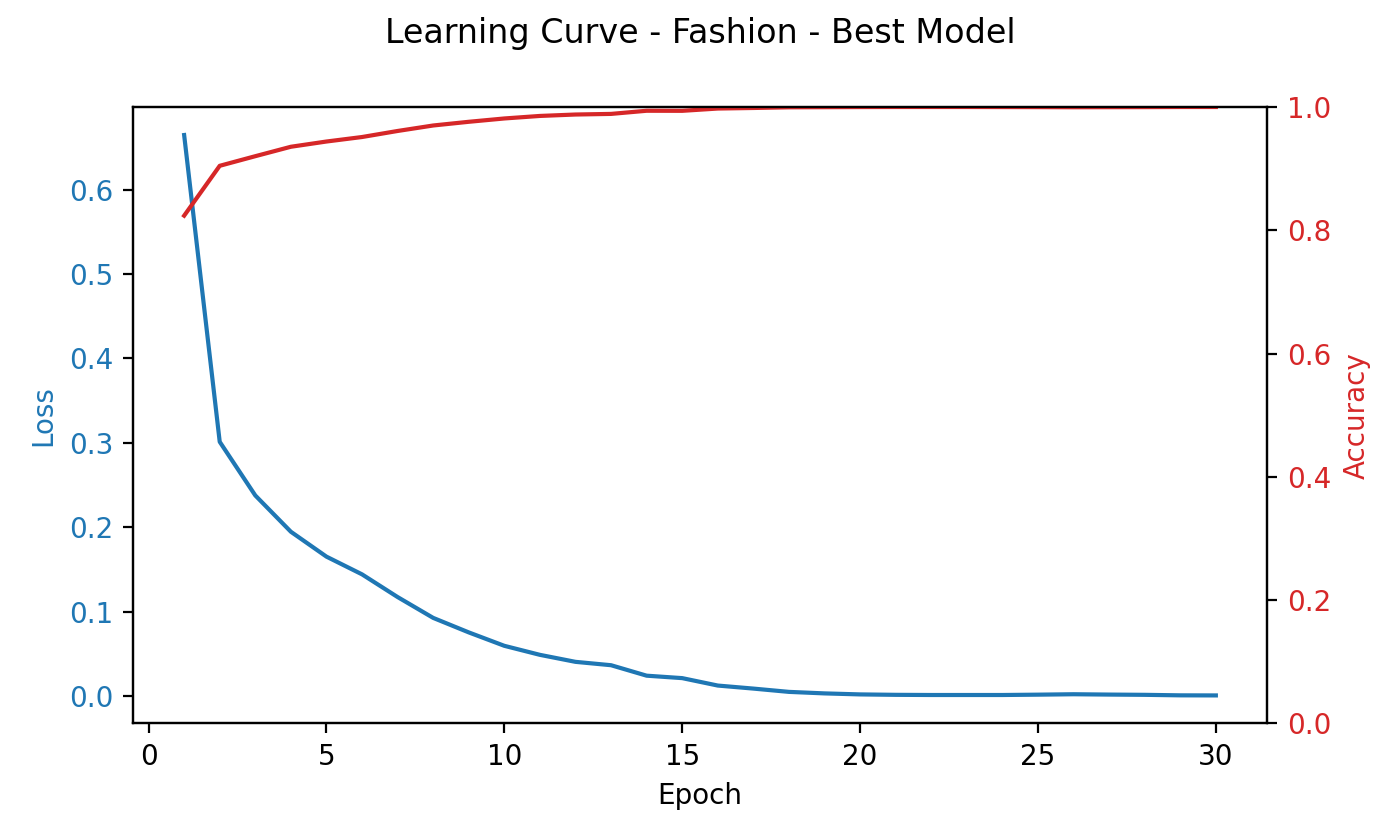
\includegraphics[width=\linewidth]{learning_curve_fashion_best.png}
        \caption*{Best model}
    \end{minipage}
    \caption{Learning curve (Loss/Accuracy) cho Fashion MNIST: strong baseline vs. best model}
    \label{fig:fashion-learning-curve}
\end{figure}

\begin{figure}[H]
    \centering
    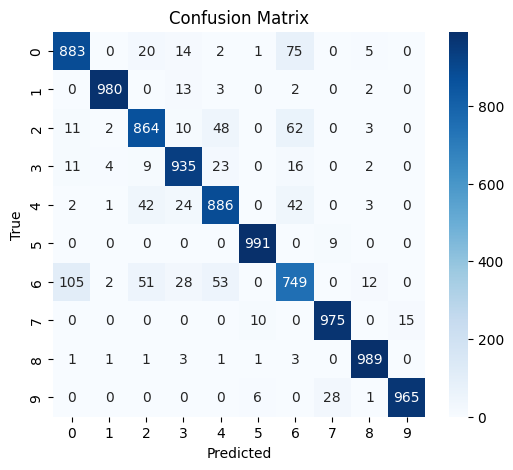
\includegraphics[width=0.6\linewidth]{ann_confusion_matrix_best_fashion.png}
    \caption{Ma trận nhầm lẫn của mô hình tốt nhất cho Fashion MNIST}
    \label{fig:fashion-cm-best}
\end{figure}

\subsection{PneumoniaMNIST}
\subsubsection{Phân tích kết quả}
Vanilla Baseline (không BatchNorm/Dropout) đạt 0.8349. Trong notebook enhance, Strong Baseline có BatchNorm sau từng Linear (fc1, fc2, fc3) và Dropout ngay sau ReLU đạt 0.8878. Do dữ liệu bị lệch giữa hai lớp, Accuracy không đủ phản ánh toàn bộ chất lượng; confusion matrix cho thấy mô hình còn nhầm một lượng đáng kể ảnh normal thành pneumonia, phản ánh xu hướng thiên về dự đoán lớp bệnh (xem Hình~\ref{fig:med-cm-baseline}).

\begin{figure}[H]
    \centering
    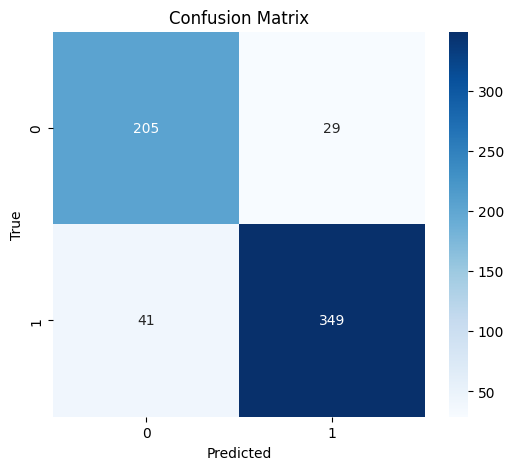
\includegraphics[width=0.55\linewidth]{ann_baseline_cm_med.png}
    \caption{Ma trận nhầm lẫn của mô hình baseline cho PneumoniaMNIST}
    \label{fig:med-cm-baseline}
\end{figure}

\subsubsection{Động lực cải tiến}
Từ EDA, PneumoniaMNIST có mất cân bằng lớp và tín hiệu phân biệt thiên về cấu trúc hơn là hình dáng. Vì vậy nhóm thử hai hướng: (1) feature engineering để làm nổi bật cấu trúc cục bộ hoặc tương phản (HOG, CLAHE, CLAHE+HOG), và (2) loss engineering bằng weighted loss để cân bằng Precision/Recall. Augmentation được thử nhưng cần thận trọng vì ảnh y khoa ít phù hợp với biến đổi hình học mạnh.

\textbf{Thông số augmentation (Pneumonia):} RandomRotation $\pm 5^{\circ}$ và ColorJitter (brightness $\pm 0.1$, contrast $\pm 0.1$). Với Digit, xoay $\pm 10^{\circ}$ phản ánh đúng nét viết tay nghiêng tự nhiên. Nhưng với Pneumonia, ảnh X-quang thường được chụp cố định trên giá đỡ bệnh viện; việc ép mô hình học các ảnh bị xoay dù chỉ $\pm 5^{\circ}$ kèm thay đổi độ sáng/tương phản đã đưa vào nhiễu loạn phi thực tế, dẫn đến độ chính xác giảm xuống 0.8446.

\subsubsection{Cải tiến và kết quả}
\textbf{Bảng tổng hợp cải tiến (từ notebook clean)}
\begin{table}[H]
    \centering
    \caption{Kết quả các cải tiến trên PneumoniaMNIST}
    \label{tab:pneumonia-improvements}
    \begin{tabular}{lrrrr}
        \toprule
        \textbf{Phương pháp} & \textbf{Accuracy} & \textbf{F1} & \textbf{Precision} & \textbf{Recall} \\
        \midrule
        Raw & 0.8878 & 0.8883 & 0.8896 & 0.8878 \\
        Augmentation & 0.8446 & 0.8346 & 0.8667 & 0.8446 \\
        HOG & \textbf{0.8958} & \textbf{0.8927} & \textbf{0.9035} & \textbf{0.8958} \\
        CLAHE & 0.8157 & 0.7980 & 0.8553 & 0.8157 \\
        CLAHE + HOG & 0.8253 & 0.8153 & 0.8396 & 0.8253 \\
        Weighted Loss & 0.8894 & 0.8855 & 0.8992 & 0.8894 \\
        HOG + Weighted Loss & 0.8942 & 0.8914 & 0.8998 & 0.8942 \\
        \bottomrule
    \end{tabular}
\end{table}

\begin{figure}[H]
    \centering
    \begin{minipage}{0.48\linewidth}
        \centering
        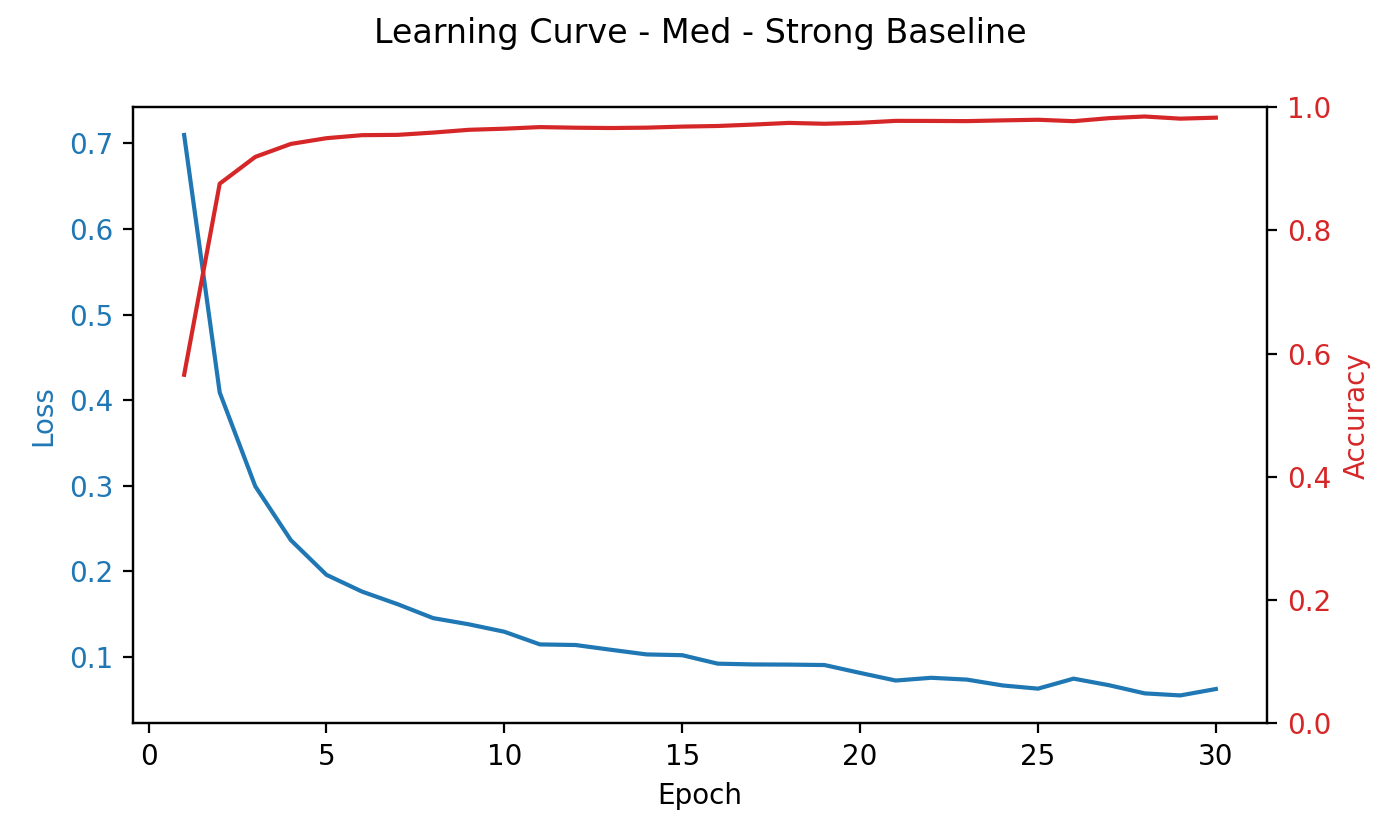
\includegraphics[width=\linewidth]{learning_curve_med_strong.png}
        \caption*{Strong baseline}
    \end{minipage}
    \hfill
    \begin{minipage}{0.48\linewidth}
        \centering
        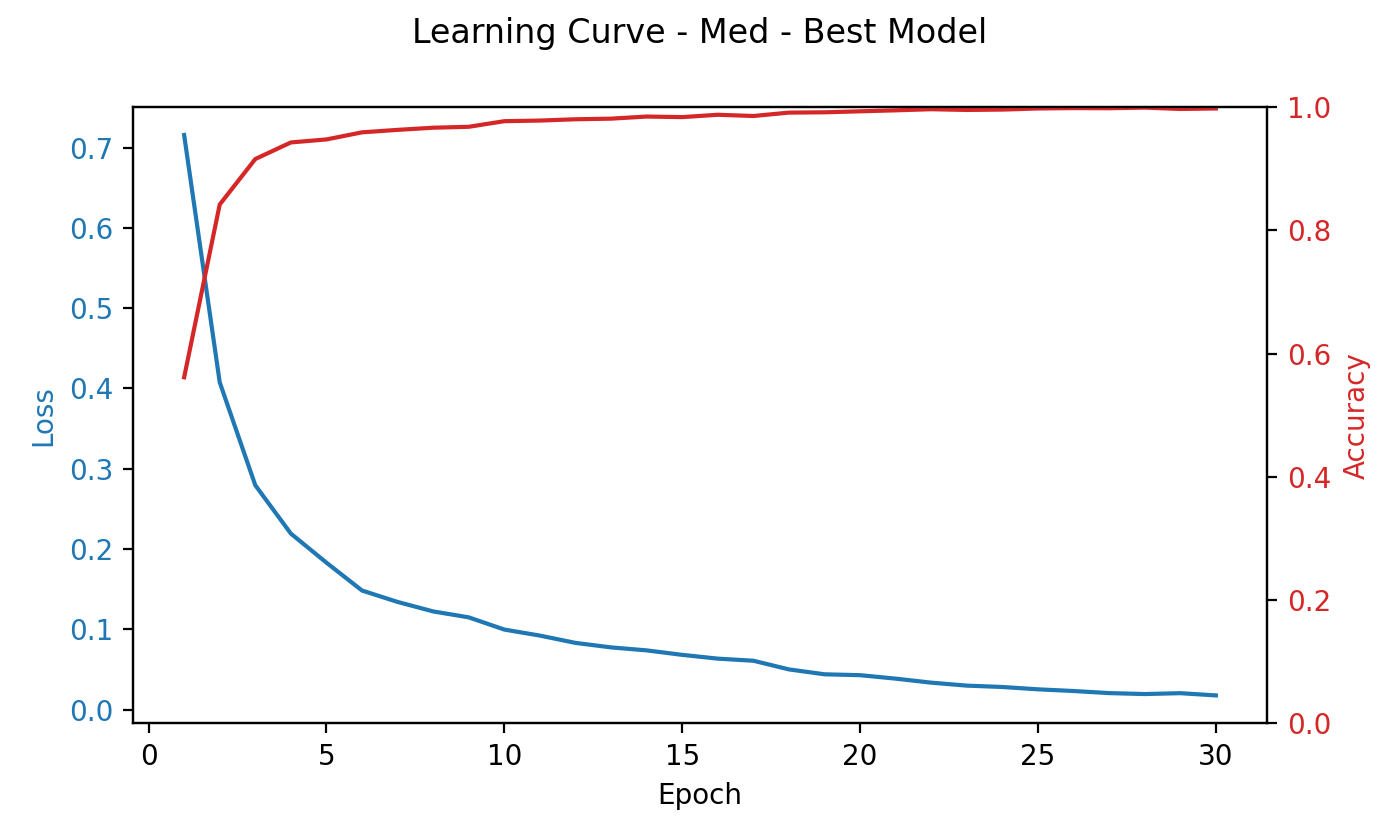
\includegraphics[width=\linewidth]{learning_curve_med_best.png}
        \caption*{Best model}
    \end{minipage}
    \caption{Learning curve (Loss/Accuracy) cho PneumoniaMNIST: strong baseline vs. best model}
    \label{fig:med-learning-curve}
\end{figure}

\textbf{Kiến trúc sử dụng cho các cải tiến}
\begin{itemize}
    \item Với raw/augmentation/CLAHE: ANN 784 $\rightarrow$ 512 $\rightarrow$ 256 $\rightarrow$ 128 $\rightarrow$ 2 (input 784, output 2 lớp), kèm BatchNorm sau mỗi Linear và Dropout sau mỗi ReLU ở các tầng ẩn.
    \item Với HOG/CLAHE+HOG: ANN 1296 $\rightarrow$ 512 $\rightarrow$ 256 $\rightarrow$ 128 $\rightarrow$ 2 (input 1296, output 2 lớp), kèm BatchNorm và Dropout theo cùng vị trí như trên.
\end{itemize}

\subsubsection{Thảo luận}
Learning curve của PneumoniaMNIST giảm chậm và có dao động nhẹ, phản ánh dữ liệu nhỏ và lệch lớp. Best model cải thiện plateau nhưng chênh lệch không lớn, phù hợp với nhận xét về độ bất định thống kê trên tập test nhỏ.
\begin{itemize}
    \item HOG là cải tiến tốt nhất theo Accuracy trong các thử nghiệm ở notebook clean (0.8958).\footnote{skimage.feature.hog: \href{https://scikit-image.org/docs/stable/api/skimage.feature.html\#skimage.feature.hog}{https://scikit-image.org/docs/stable/api/skimage.feature.html}}
    \item Weighted loss giúp cân bằng Precision/Recall; kết hợp HOG + weighted loss cho kết quả ổn định và gần với HOG thuần.
    \item CLAHE và CLAHE + HOG không mang lại cải thiện rõ; tăng tương phản cục bộ có thể làm nổi cả nhiễu.
\end{itemize}

\begin{figure}[H]
    \centering
    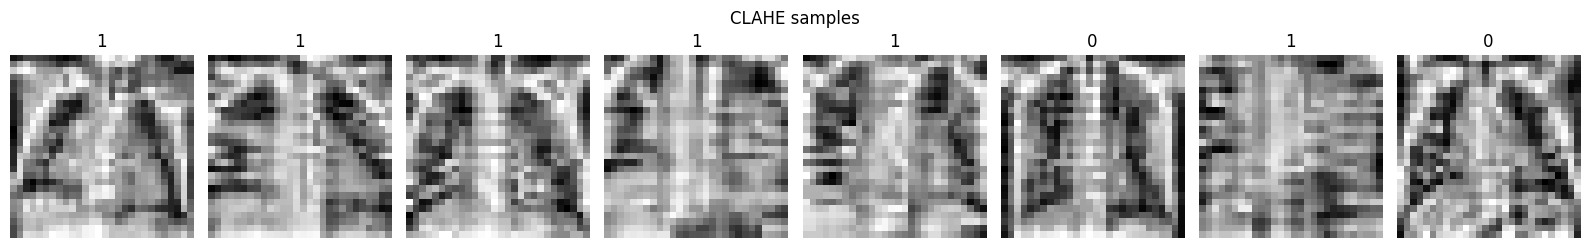
\includegraphics[width=0.9\linewidth]{ann_med_contrast_clahe_samples.png}
    \caption{Ví dụ ảnh PneumoniaMNIST sau CLAHE}
    \label{fig:med-clahe-samples}
\end{figure}

\begin{figure}[H]
    \centering
    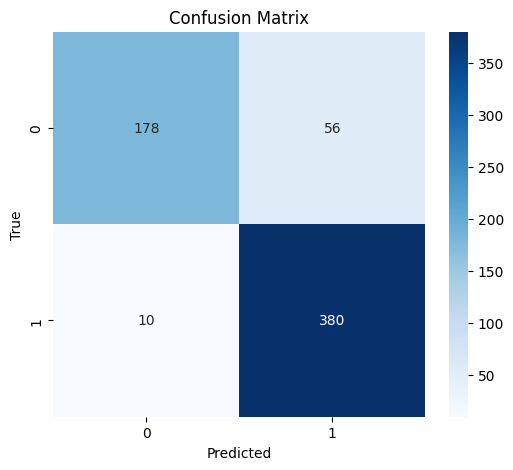
\includegraphics[width=0.55\linewidth]{ann_confusion_matrix_best_med.png}
    \caption{Ma trận nhầm lẫn của mô hình tốt nhất cho PneumoniaMNIST}
    \label{fig:med-cm-best}
\end{figure}



\section{So sánh kết quả}
\subsection{Bảng tổng hợp}
\begin{table}[H]
    \centering
    \caption{So sánh Vanilla Baseline và cải tiến tốt nhất theo Accuracy và F1}
    \label{tab:compare-best}
    \begin{tabular}{lrrrrr}
        \toprule
        \textbf{Dataset} & \textbf{B-Acc} & \textbf{B-F1} & \textbf{Best-Acc} & \textbf{Best-F1} & \textbf{Best Method} \\
        \midrule
        Digit MNIST & 0.9438 & 0.9437 & \textbf{0.9939} & \textbf{0.9939} & HOG + Aug + BN \\
        Fashion MNIST & 0.8443 & 0.8425 & \textbf{0.9217} & \textbf{0.9213} & HOG \\
        PneumoniaMNIST & 0.8349 & 0.8817 & \textbf{0.8958} & \textbf{0.8927} & HOG \\
        \bottomrule
    \end{tabular}
\end{table}

\subsection{Phân tích}

\begin{itemize}
    \item \textbf{Nhận xét 1:} Khi dữ liệu thiên về hình dạng rõ ràng (Digit, Fashion), đặc trưng dựa trên gradient như HOG rất hiệu quả.
    
    \item \textbf{Nhận xét 2:} Data augmentation chỉ hữu ích khi phản ánh đúng biến thiên tự nhiên của dữ liệu; nếu không, có thể làm lệch phân bố và giảm hiệu quả.
    
    \item \textbf{Nhận xét 3:} Với dữ liệu y khoa lệch lớp, cần theo dõi F1/Recall và cân bằng loss; accuracy đơn thuần không đủ để đánh giá. Mặc dù mô hình Weighted Loss có Accuracy thấp hơn HOG một chút (0.8894 vs 0.8958), nhưng nó mang lại sự cân bằng tốt nhất giữa việc phát hiện đúng bệnh nhân (Recall) và không báo động giả (Precision), đây mới là yếu tố quyết định trong y khoa.

    \item \textbf{Nhận xét 4 (bẫy thống kê):} Sự chênh lệch giữa Raw (0.8878) và HOG (0.8958) trên tập Pneumonia test chỉ tương đương khoảng 5 mẫu dự đoán đúng. Do kích thước tập test khá nhỏ ($N=624$), sự vượt trội này chưa mang ý nghĩa thống kê chắc chắn; cần thử nghiệm trên tập dữ liệu y khoa lớn hơn để khẳng định ưu thế của HOG trong việc trích xuất kết cấu X-quang.
\end{itemize}

\section{Kết luận}
\begin{itemize}
    \item ANN phù hợp nhất với Digit MNIST, khá tốt với Fashion MNIST, và hạn chế với PneumoniaMNIST do texture phức tạp và mất cân bằng lớp.
    \item Giới hạn chính của ANN là mất thông tin không gian khi flatten và nhạy với mất cân bằng lớp.
    \item Hướng mở rộng: dùng CNN, tăng cường dữ liệu có kiểm soát, weighted loss/metrics theo lớp, và thử mô hình học đặc trưng chuyên sâu cho ảnh y khoa.
\end{itemize}

\end{document}